\section*{UDL, Teaching Practice, and Student Vulnerability -- Connecting the Issue to the Present}

\begin{wrapfigure}{l}{0.5\textwidth}
\vspace{-2em}
\centering
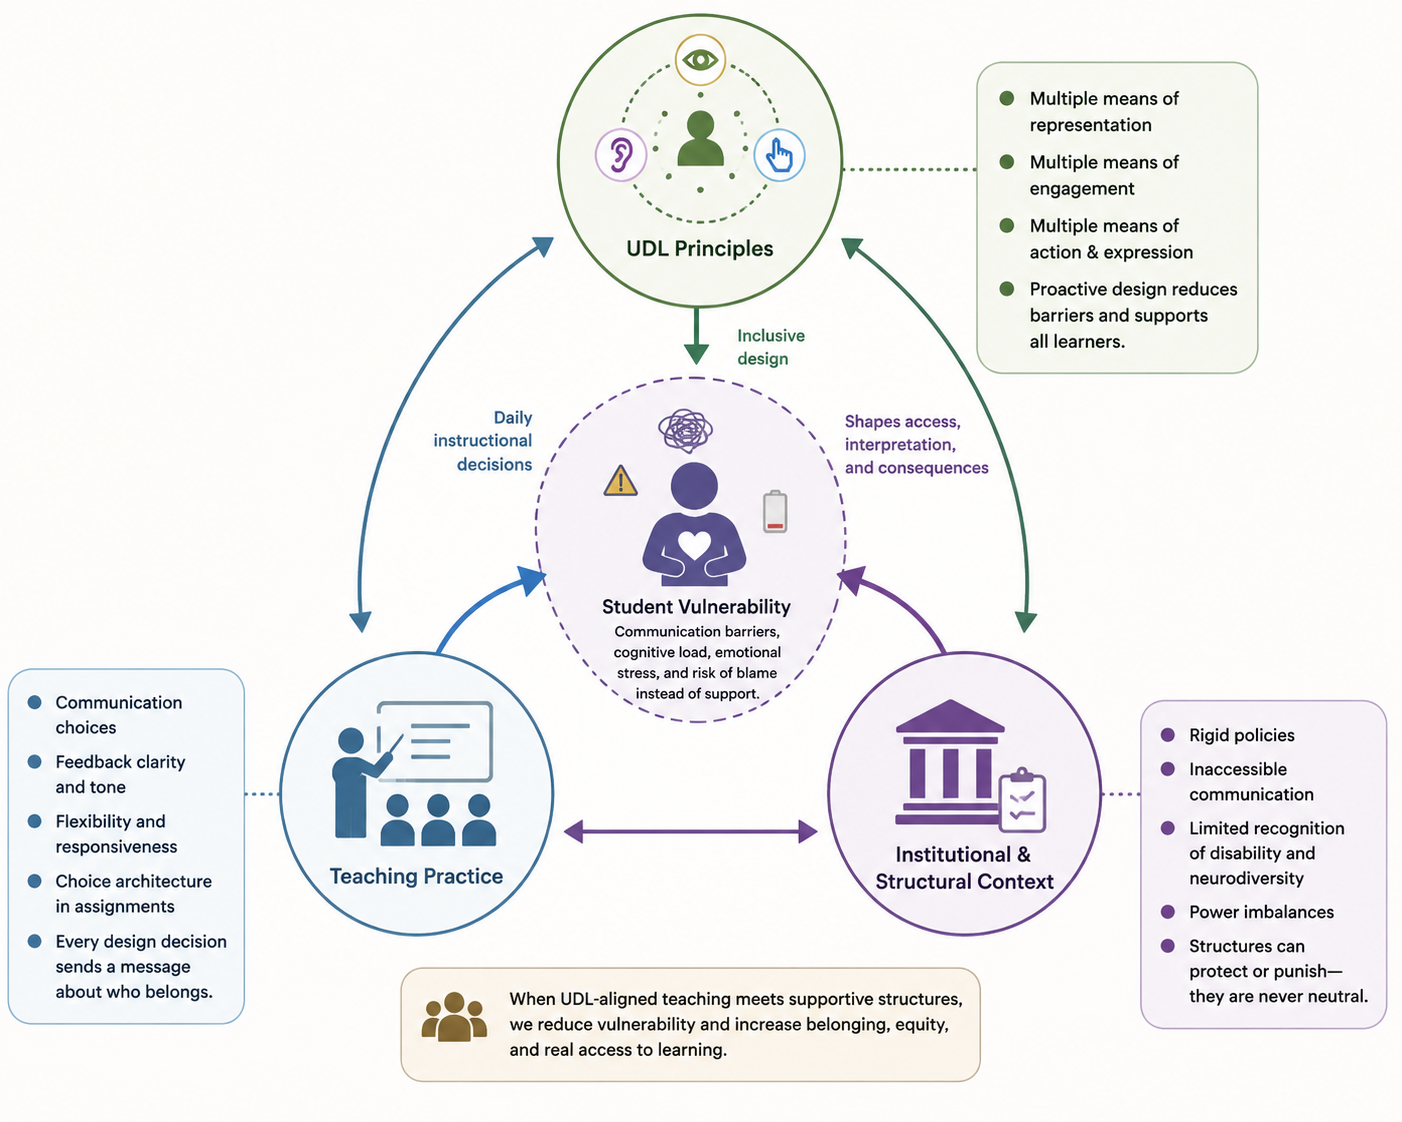
\includegraphics[
width=0.5\textwidth,
height=0.5\textheight,
keepaspectratio,
% trim=1.2cm 0.4cm 1.2cm 0.3cm,
% clip
]{images/connecting_issues_to_the_present.png}

{\scriptsize\textit{Figure 6. This visual shows how UDL, teaching practice, and institutional structures shape student vulnerability. It emphasizes that vulnerability is not only located in the student; it is intensified or reduced by the design of communication, flexibility, feedback, and support.}\par}

\vspace{-1em}
\end{wrapfigure}

A present-day initiative that directly connects to this issue is \textit{Universal Design for Learning} (UDL), especially the \textit{CAST UDL Guidelines 3.0}. UDL shifts the question from \textit{How do we help students after they struggle?} to \textit{How do we design learning environments so access is built in from the beginning?} CAST describes the UDL Guidelines as a framework that can be applied across disciplines so learners can access and participate in meaningful, challenging learning opportunities. The current Guidelines 3.0 also name \textit{learner agency as the goal}: learners who are purposeful and reflective, resourceful and authentic, and strategic and action-oriented \citep{cast2024udl}.

This connects directly to communication-access injustice because many classroom harms begin before a student ever fails an assignment. They begin with how expectations are communicated, how language is defined, how feedback is delivered, how accommodations are framed, how students are invited to participate, and how much flexibility exists for students whose bodies and brains do not match the assumed classroom norm. \textit{UDL provides a present-day framework for redesigning those conditions.}

% \subsection*{Target Audience}

The target audience for UDL includes teachers, professors, curriculum designers, instructional designers, researchers, families, and educational support systems. For this paper, I focus especially on teachers and professors because they make daily communication decisions that shape access. They decide whether instructions are spoken, written, modeled, repeated, and findable. \textit{They decide whether assignment expectations are stable and accessible}, whether technical language is modeled or assumed, and whether \textit{accommodations are treated as a burden}, a legal minimum, or a doorway into better design.

Students are also part of this audience, but they should not be the only ones responsible for access. A neurodivergent or chronically ill student should not have to become an expert in disability services, institutional language, professor communication, team management, and self-advocacy just to survive a course. Children are even more vulnerable because \textit{they often do not have the language, confidence, or institutional power to explain when a classroom system is inaccessible}.

% \subsection*{Expected Literacy Levels}

This issue cannot be understood through a simple high-literacy or low-literacy framework. Students and educators bring different kinds of literacy to the classroom. A student may have advanced scientific literacy but limited institutional literacy. They may understand bioinformatics concepts but not know how to interpret accommodation procedures, grading policies, or escalation pathways. A neurodivergent student may have strong analytical literacy but need stable written expectations and explicit sequencing. A chronically ill student may understand the course content but need communication systems that account for unpredictable capacity. A multilingual or culturally and linguistically diverse student may understand the concept but be excluded by unexplained academic language, idioms, or institutional phrasing. A child may understand an idea deeply through building, drawing, movement, or peer explanation, but still be marked as confused if the classroom only recognizes one approved way of showing knowledge.

UDL is useful because it recognizes learner variability as normal rather than exceptional. \textit{The Guidelines include design options for clarifying vocabulary and language structures, supporting multiple ways to perceive information}, using multiple media for communication, organizing information and resources, fostering belonging and community, and challenging exclusionary practices \citep{cast2024udl}.

% \subsection*{Accessibility Strategies Used by UDL}

UDL offers accessibility strategies that directly respond to the communication barriers named in this paper. First, UDL emphasizes \textit{multiple means of representation}. Students should not have to depend on one spoken explanation, one written paragraph, or one hidden expectation. Important information should be available through stable written instructions, visual models, examples, discussion, demonstration, and opportunities for clarification.

Second, UDL emphasizes \textit{language and symbols}. CAST includes guidance to clarify vocabulary, support decoding, cultivate understanding across languages and dialects, address bias in language, and illustrate through multiple media \citep{cast2024udl}. This connects directly to the BIO/STEM case because scientific, institutional, and grading language can become exclusionary when treated as obvious.

Third, UDL emphasizes \textit{action and expression}. Students should have multiple ways to communicate what they know, use tools, build fluency, and demonstrate learning. This matters for neurodivergent, chronically ill, and K--12 students because knowledge does not always appear through one approved format. A student may show understanding through writing, speaking, coding, building, drawing, explaining to a peer, revising, or physically manipulating materials.

Finally, UDL emphasizes \textit{belonging, collaboration, emotional capacity, and learner agency}. A student who feels threatened, shamed, confused, or punished for needing clarification cannot fully participate. CAST Guidelines 3.0 explicitly respond to barriers rooted in bias and systems of exclusion \citep{cast2024udl}.

% \subsection*{Potential Communication Barriers}

UDL is powerful, but \textit{it can still become abstract if educators do not treat it as a communication practice.} A professor may agree with UDL in principle while still relying on single-mode instructions, unclear policies, inaccessible grading language, or accommodation communication that feels like compliance rather than care. One barrier is \textit{professional abstraction}; terms like learner agency, representation, engagement, and action and expression are meaningful, but they can become jargon if teachers are not shown how to translate them into daily classroom decisions. For example, multiple means of representation must become concrete actions: written directions, visual examples, posted changes, explicit vocabulary, stable deadlines, and accessible feedback.

Another barrier is \textit{digital access}. UDL resources are often online, which can support broad access, but digital platforms may still exclude families, teachers, or students with limited internet access, limited technological literacy, language barriers, or disabilities affecting navigation. A third barrier is \textit{implementation without accountability}. A school or \textit{professor can claim to value accessibility without changing the systems that create harm}. UDL only matters if it changes how communication is designed, expectations are clarified, students are allowed to participate, and educators respond when students say they cannot access the learning environment.

% \subsection*{Connection to Teaching Practice}

My teaching-placement observations make this issue even more urgent. Children often show understanding through movement, building, drawing, experimenting, peer teaching, repetition, and guided practice. They may not have the words to explain what kind of support they need, but their behavior often communicates it. When a student shuts down, rushes, avoids, interrupts, or keeps asking the same question, the issue may not be a lack of ability. It may be a communication-access issue.

\begin{wrapfigure}{r}{0.5\textwidth}
\vspace{-4em}
\centering
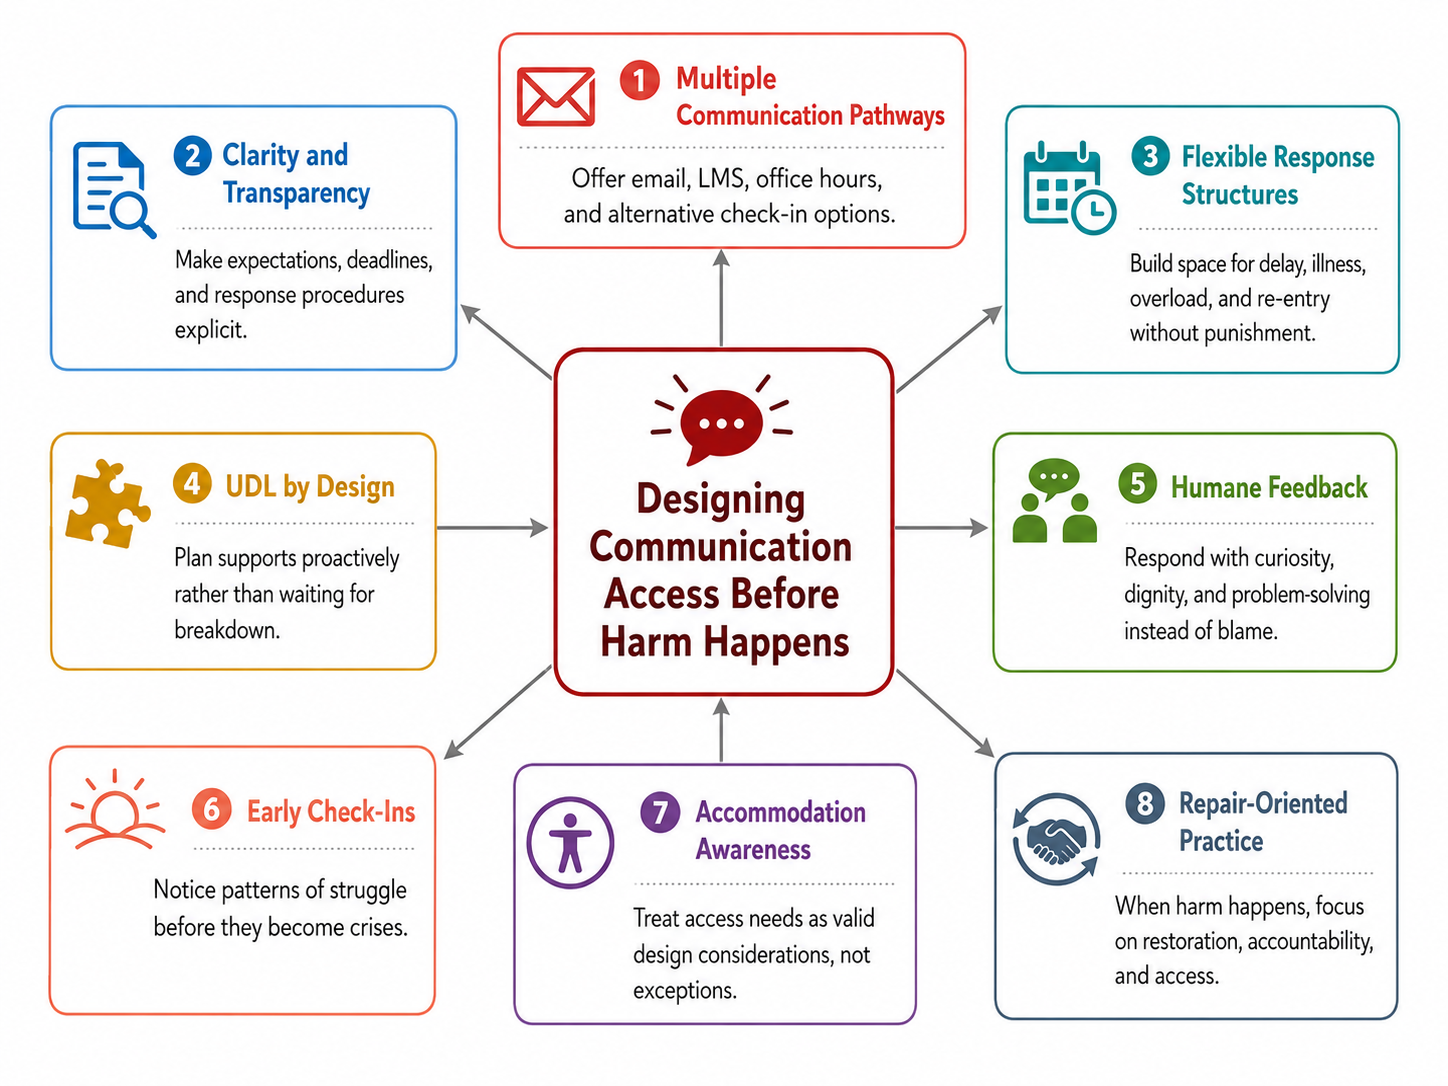
\includegraphics[
width=0.5\textwidth,
height=0.5\textheight,
keepaspectratio,
% trim=1.5cm 0.5cm 1.5cm 0.5cm,
% clip
]{images/designing_communication_access.png}

{\scriptsize\textit{Figure 7. This summarizes recommendations for designing access before harm happens. It shows how multiple communication pathways, clear expectations, flexible response structures, UDL-based supports, humane feedback, early check-ins, accommodation awareness, and repair-oriented practice can reduce barriers.}\par}

\vspace{-3em}
\end{wrapfigure}

This is why the adult BIO/STEM evidence matters beyond one course. It shows what happens when an adult with documentation skills, technical expertise, and support still has to fight the system. In K--12 settings, many students cannot fight that way. They need teachers to design access before the breakdown happens. UDL gives educators a way to do that. It asks teachers to expect variability, clarify language, offer multiple pathways, support agency, and challenge exclusionary practices. In the context of this paper, UDL becomes more than an accessibility framework. It becomes a social justice response to the communication systems that decide whether students are understood, supported, and allowed to belong.


\section*{Recommendations -- Designing Communication Access Before Harm Happens}

The recommendations are based on a central claim: \textit{communication access should be designed before students are harmed}, not repaired after students break down, fall behind, or are forced to advocate under pressure. A classroom cannot be socially just if students must decode hidden expectations, translate illness into institutional language, or \textit{prove that their access needs are legitimate} before they are allowed to participate fully. These recommendations do not lower academic standards but make them clearer, more stable and humane. In STEM especially, rigor should mean meaningful disciplinary challenge. \textit{A course can ask students to do complex work while still making expectations visible}, language teachable, feedback accessible, and participation flexible.

% \subsection*{Make Requirements Stable, Written, and Findable}

\textit{The first recommendation is that all graded expectations should be written in a stable, centralized location.} If a requirement affects grading, participation, submission format, or peer evaluation, it \textit{should not depend on memory for oral directions or informal clarification}. Students should be able to find the requirement after class, review it when symptoms or executive-function barriers interfere, and verify it without having to ask whether they missed something. \textit{This means instructors should provide assignment summaries in plain language, written versions of important verbal updates, examples of successful submissions, clear grading criteria, visible revision or feedback policies, and an explicit communication-channel hierarchy.} For example, a course should clearly identify where official instructions live: syllabus, learning management system, assignment page, email, or shared document. If an instruction changes, the change should be posted in the same official location. This helps all students, but it is especially important for neurodivergent students, ill students, multilingual students, and students who rely on written records to manage cognitive load.

% \subsection*{Treat Accommodations as a Design Floor, Not a Ceiling}

The second recommendation is that \textit{accommodations should be treated as the beginning of access design}, not the full extent of it. Disability accommodations are important, but they often operate after a student has already had to disclose, document, request, and negotiate support. \textit{A socially just classroom should not wait for formal accommodation letters before designing communication that is clear, flexible, and accessible}. Instructors should ask which parts of the course require unnecessary memory, which expectations are hidden or implied, \textit{which policies would be difficult to interpret during illness or executive-function overload}, which communication systems assume that all students process information in the same way, and which supports could be built into the course for everyone. \textit{This approach protects students who have formal accommodations}, but it also supports students who are undiagnosed, newly diagnosed, culturally hesitant to disclose, temporarily ill, grieving, traumatized, multilingual, or unsure how to ask for help.

% \subsection*{Teach Disciplinary Language Explicitly}

The third recommendation is to teach \textit{disciplinary language as part of the course}. In bioinformatics and computer science, students are not only learning content but also how to read scientific language, technical documentation, code, file formats, workflows, and data conventions. Specialized language should not be removed from STEM. Students need access to disciplinary language to enter the field, but that language should be modeled, defined, revisited, and connected to examples. This can include short vocabulary bridges before technical tasks, annotated examples of reports and data files, visual workflow maps, glossary links, side-by-side plain-language and disciplinary-language explanations, and opportunities to ask terminology questions without shame. \textit{This recommendation matters because disciplinary literacy can either open the door to STEM or become another gatekeeping mechanism.}

% \subsection*{Build Communication Norms Into Teamwork}

The fourth recommendation is to \textit{make team communication expectations explicit before conflict occurs}. Group work is often treated as automatically inclusive because students are working together, but \textit{collaboration can become inaccessible} when roles, tools, deadlines, decision-making norms, and conflict processes are unclear. Courses that require teamwork should include written team-role expectations, shared norms for communication platforms, expectations for documenting decisions, protocols for missed meetings or illness, peer-evaluation criteria explained in advance, private support pathways when team dynamics become harmful, and instructor \textit{check-ins that focus on process} rather than only product. This is especially important for students whose access needs affect timing, communication style, energy, memory, or emotional regulation. Teamwork should not depend on students privately negotiating disability, illness, or conflict without support.

% \subsection*{Use Multiple Modes of Communication and Expression}

The fifth recommendation is to design multiple pathways for receiving information and demonstrating learning. Students should not be limited to one mode of access or expression when the learning goal could be met in more than one way. In practice, this means pairing spoken directions with written directions, written instructions with visual examples, technical vocabulary with plain-language explanations, feedback comments with examples, individual work with structured collaboration, and formal writing with diagrams, code, demonstrations, oral explanations, or design artifacts where appropriate. This recommendation connects directly to Universal Design for Learning. Multiple modes do not weaken learning but make it more visible. They allow students to show understanding without being blocked by a single communication format.

% \subsection*{Create Student-Facing Institutional Literacy Supports}

The sixth recommendation is to \textit{make institutional pathways easier} to understand before students are in crisis. Students should not have to discover disability services, Ombuds, advising, escalation procedures, grade policies, or withdrawal options only after harm has already occurred. Schools and instructors can support institutional literacy by providing a plain-language guide to support offices, a short explanation of when to contact each office, examples of what students can say when asking for help, links to accommodation and conflict-resolution processes, reminders that seeking help is responsible rather than disruptive, and private ways to ask for clarification. This matters because institutional literacy is unevenly distributed. Adult graduate students may learn how to navigate systems over time. Children, first-generation students, multilingual students, disabled students, and students in crisis may not have that knowledge yet.

% \subsection*{Build Community Dialogue Into Course Design}

The final recommendation is to create \textit{classroom cultures where students can talk about access} before conflict or failure. Communication access is not only a technical design problem, but also relational. Students need to know that clarification is welcome, that confusion will not be punished, and that difference will not be treated as inconvenience. Community dialogue can include beginning-of-course access check-ins, anonymous feedback forms, class norms around asking questions, opportunities to name confusing language, structured reflection on how students learn best, instructor modeling of revision and clarification, and explicit statements that \textit{access needs are part of learning design.} This is especially important in classrooms with neurodivergent, chronically ill, disabled, culturally and linguistically diverse, multilingual, trauma-impacted, anxious, or depressed students. \textit{These students should not have to become visible only when something goes wrong.}

% \subsection*{Closing Recommendation}

The larger recommendation is a shift from accommodation as exception to communication access as design. Instructors should not ask, \textit{"What is wrong with this student that they cannot follow the course?"} They should ask, \textit{"What does this course require students to decode, remember, perform, or navigate before they can show what they know?"} That question changes the responsibility; it does not remove student accountability, but it places educator accountability where it belongs, in the design of the learning environment. A socially just classroom makes expectations visible, language accessible, participation flexible, and support pathways clear. \textit{It does not ask students to break themselves, proving that they deserved access all along.}
\section*{From Pain to Protection -- A Critical Reflection}

This paper forced me to look at literacy in a way that is both academic and personal. Before this course, I would have described literacy mostly through reading, writing, language, and communication. I still believe those matter, but this assignment helped me see literacy as something larger: the ability to access the systems that decide whether a person is understood, included, believed, and allowed to participate.

That realization changed how I understood the BIO/STEM communication-access evidence. At first, it could look like a conflict or misunderstanding. Through the lens of literacy and social justice, I saw something deeper. The issue was not only whether one instruction was clear or unclear. The issue was how much of the course required students to decode expectations, interpret authority, manage institutional language, navigate accommodations and team relationships, and translate illness into acceptable academic communication. That is literacy. Because not every student has equal access to those forms of literacy, it is also power.

The most painful part of this reflection is that I was not a child when this happened. I was an adult graduate student with technical knowledge, documentation habits, advisor support, and experience advocating for myself. I had language for disability, chronic illness, neurodivergence, and institutional processes. Even with all of that, the communication system still affected my health, confidence, sense of belonging, and ability to participate fully.

That is why I cannot treat this as only my story. If this can happen to an adult with resources, then I have to ask, \textit{what happens to students who do not have those resources?} What happens to children who cannot explain that an expectation was inaccessible? What happens to multilingual students who understand the concept but not the institutional language around it? What happens to chronically ill students who are already exhausted before they begin the work of self-advocacy? \textit{What happens to neurodivergent students whose need for clarity is mistaken for resistance, carelessness, or immaturity?}

This assignment helped me understand that literacy can either protect students or expose them to harm. When expectations are clear, language is taught, feedback is accessible, and support pathways are visible, literacy becomes empowering. It gives students a way into the classroom. But \textit{when expectations are hidden, terminology is assumed, accommodations are treated as limits, and students are expected to interpret systems alone, literacy becomes a barrier}. It rewards students who already know how to navigate the system and punishes those who need the system to be explained.

The connection to my teaching placement made this even clearer. Children often show understanding through movement, building, drawing, repetition, peer teaching, experimentation, and emotional response. They do not always have the words to say, \textit{the communication structure is not accessible to me}. Instead, they show us through behavior. They ask again, freeze, rush, avoid, interrupt, copy a peer, or act like they do not care when they may actually care deeply.

As a teacher, that changes my responsibility. I cannot wait until a student fails before asking whether the directions were accessible. \textit{I cannot wait until a student has a diagnosis before designing for variability.} I cannot assume that a quiet student understands or that a frustrated student is refusing. I have to build \textit{communication that makes expectations visible, language teachable, participation flexible, and clarification safe}.

Universal Design for Learning gives one way to do that, but this project also taught me that \textit{frameworks only matter if they become practice}. It is easy to say that we value multiple means of representation, engagement, and expression. It is harder to ask whether the syllabus, assignment instructions, grading policies, feedback systems, and team expectations actually reflect those values. \textit{Accessibility is a design decision repeated every day.}

This reflection also connects to my larger work in equity and AI. In my research, I often think about systems that make decisions based on incomplete, biased, or poorly designed data. This project reminded me that classrooms can do the same thing. A student can be misclassified by a teacher just as a patient can be misclassified by an algorithm. \textit{A system can appear neutral while still reproducing harm.} A policy can seem objective while still excluding the people it was never designed to understand.

That is why I see this paper as more than a course assignment. It is part of a larger commitment to diagnostic justice, educational justice, and communication design. Whether I am working in a classroom, a bioinformatics system, or an AI framework, the question is similar: \textit{who is being misread by the system, and what would it take to design the system so they are seen more accurately?}

The answer begins with literacy. Not literacy as a narrow measure of skill, but \textit{literacy as access, identity, agency, and recognition}. Students should not have to break themselves to prove that they are capable. They should not have to become experts in hidden rules before they are allowed to learn. They should not have to translate pain into perfect institutional language before they are believed.

For me, the purpose of this project is protection. I am writing from my own experience, but I am not writing only for myself. \textit{I am writing for the students who will come after me}, especially the ones who are younger, quieter, sicker, more scared, less resourced, or less able to name what is happening to them. Communication access is the doorway into learning. When that doorway is narrow, hidden, or guarded by assumptions, students are excluded before they ever get a chance to show who they are. A just classroom widens that doorway. It does not lower the destination; it makes the path visible.
